\clearpage
\section{Setting the boards in the appropriate MODE} \label{sec:modes}

%%%%%%%%%%%%%%%%%%%%%%%%%%%%%%%%%%%%%%%%%%%%%%%%%%%%%%%%%%%%%%%%%%%%%%%%%%%%%%%%%%%%
\subsection{Development mode: powered by USB (ST-LINK)} \label{sec:mode-dev}

This mode is the one that you will use the most during this project. Good point, as it is the more convenient! You can basically do everything you need in this mode by simply connecting the \texttt{STM32} board to your computer through USB. It will allow you to power all the boards, program the MCU and debug it and finally receive data from the MCU through the UART interface. For this reason, it is called \textit{Development mode} as it is the one you must use to develop your project.

\textbf{In order not to damage the boards}, you need to make sure the following settings are properly set on your hardware:

\begin{itemize}
    \item First, make sure that all jumpers shown in red in Fig \ref{fig:settings-mode-dev} are configured as in the Figure. There is nothing to set on the radio board.
    \item Then, plug in your USB-micro cable as shown in Fig. \ref{fig:settings-mode-dev}. This USB port is the one to use for the ST-LINK. The USB port at the opposite of the board is an interface for the MCU but we will not use it in this project.
    \item Finally, plug in the USB-A in your computer. The "PWR LED" (yellow-green) should be ON.
\end{itemize}

\begin{figure}[h!]
    \centering
    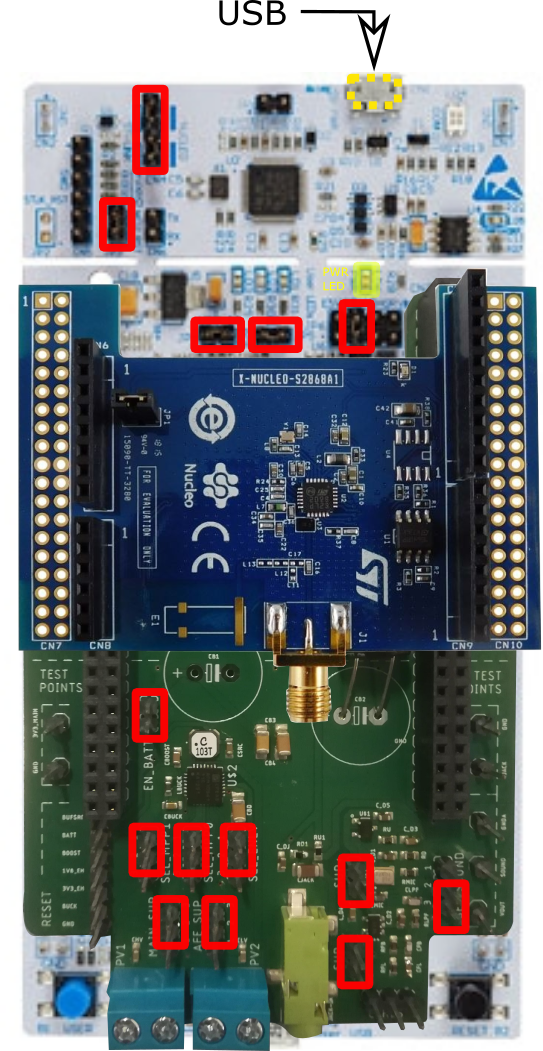
\includegraphics[width=0.4\textwidth]{figs/settings-mode-dev.png}
    \caption{Settings for the boards, development mode.}
    \label{fig:settings-mode-dev}
\end{figure}

%%%%%%%%%%%%%%%%%%%%%%%%%%%%%%%%%%%%%%%%%%%%%%%%%%%%%%%%%%%%%%%%%%%%%%%%%%%%%%%%%%%%
\clearpage
\subsection{Power monitoring mode: powered by an external 3V3 source} \label{sec:mode-3V3}

This mode is the one that you will use to monitor the \textbf{total} power drawn by your wireless smart sensors. In this mode, you have a limited amount of functionalities: it allows you to power all the boards through the external 3V3 supply but you cannot program the MCU anymore (or even debug it!). It means that you must program your MCU in advance in the development mode and then switch to this mode. In this mode, you cannot receive data from the MCU through the UART interface either. As you might guess, this is therefore not the proper mode for developing your solution! The main purpose here is to monitor the total power needed by your device once you come up with something functional. Note that in the Hands-On H2a, you will learn how to monitor the power consumption of the MCU (only) by using a dedicated jumper on the \texttt{STM32L4A6 NUCLEO-144} MCU board. However, this mode allows you to monitor the overall power consumption of your node, which is critical to make sure it remains in the power budget.

\textbf{In order not to damage the boards}, you need to make sure the following settings are properly set on your hardware:

\begin{itemize}
    \item First, make sure that all jumpers shown in red in Fig \ref{fig:settings-mode-3V3} are configured as in the Figure.
    Be really careful for the OFF jumpers: these slots have to be open (with NO jumper). If you are not sure, please call us before powering the board. It is always a better idea to ask a question rather than damaging the boards. There is nothing to set on the radio board.
    \item Then, set your external power source on 3V3 and plug it in as shown in Fig. \ref{fig:settings-mode-3V3}. Note: if you can set a maximum current as limiter, you can choose 80 mA.
    \item Finally, turn on your external power source.
\end{itemize}

\begin{bclogo}[couleur = gray!20, arrondi = 0.2, logo=\bcattention]{BE CAREFUL}
Make sure the MAIN\_SUP jumper is OFF \textit{before} powering the boards with the external power supply.
\end{bclogo}

\begin{bclogo}[couleur = gray!20, arrondi = 0.2, logo=\bcinfo]{Going below 3V3}
By using the same setup as the one proposed in this section, you can supply your system with a voltage below 3V3. You can experience by yourself down to which voltage the system can still work (Note: decrease the supply voltage step-by-step and use the datasheets to have a rough idea of the functional range of key components i.e. MCU, ...).
\end{bclogo}

\begin{figure}[h!]
    \centering
    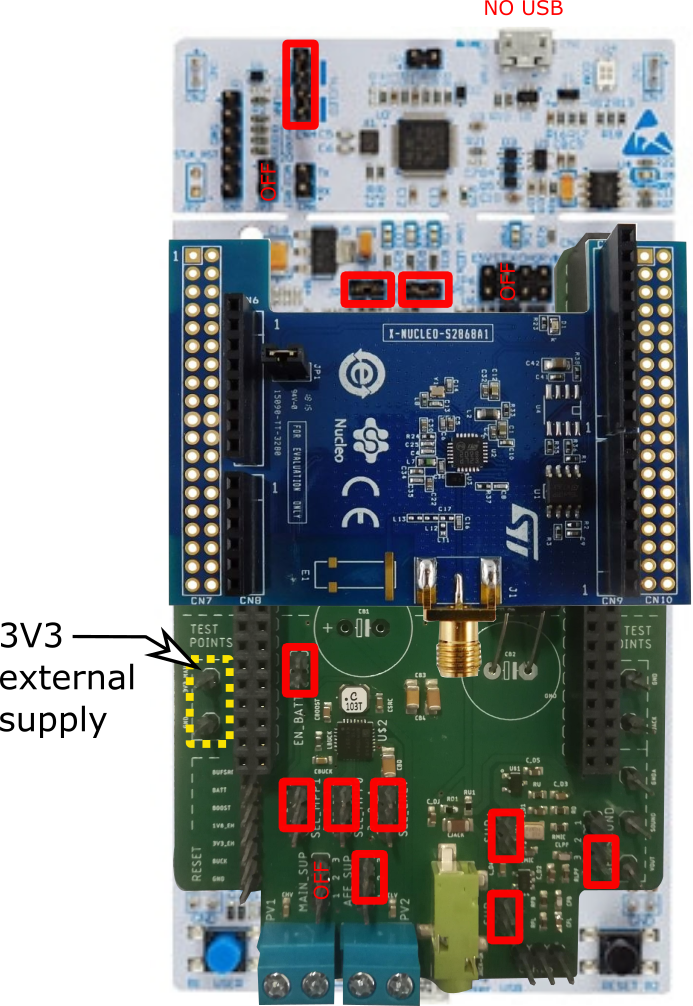
\includegraphics[width=0.5\textwidth]{figs/settings-mode-3V3.png}
    \caption{Settings for the boards, power monitoring mode.}
    \label{fig:settings-mode-3V3}
\end{figure}

%%%%%%%%%%%%%%%%%%%%%%%%%%%%%%%%%%%%%%%%%%%%%%%%%%%%%%%%%%%%%%%%%%%%%%%%%%%%%%%%%%%%
\clearpage
\subsection{Energy harvesting mode (EH): powered by PV cells} \label{sec:mode-EH}

This mode is the one that you will use to test your solution in real-world conditions: you can go full embedded by using energy harvesting of the environment thanks to the PV cells and harvesting circuitry. In this MODE, you also have a limited amount of functionalities: you cannot program the MCU anymore (or even debug it!) and you cannot receive data from the MCU through the UART interface either. Therefore, we recommend you to use this mode when (1) you have reached an advanced step of development i.e., stable and at least partially optimized; (2) you have tested in advance if your solution works in the \textit{Power monitoring mode}, see Section \ref{sec:mode-3V3}.

\textbf{In order not to damage the boards}, you need to make sure the following settings are properly set on your hardware:

\begin{itemize}
    \item First, make sure that all jumpers shown in red in Fig \ref{fig:settings-mode-eh} are configured as in the Figure.
   Be really careful for the OFF jumpers: these slots have to be open (with NO jumper). If you are not sure, please call use before powering the setting. It is always a better idea to ask a question rather than damaging the boards. There is nothing to set on the radio board.
    \item Then, plug in your PV cell(s) to harvest solar energy from the environment. Pay attention to the polarity.
    \item Finally, check out how your solution is behaving in real-life conditions!
\end{itemize}


\begin{bclogo}[couleur = gray!20, arrondi = 0.2, logo=\bcattention]{RESET procedure}
In this mode, you need to carry out a \textbf{RESET} procedure each time you want to change a setting. On the lower left part of the custom board, you have a RESET label and 7 pin headers. You need to connect each pin header to the GND pin header (the last one), starting from the first one (BUFSRC) to the sixth one (BUCK) as shown in Fig \ref{fig:reset-procedure}. Make sure you do not short two pin headers together when doing the reset procedure. Note that you can also use these pin headers to \textbf{monitor the signals} of the EH part of the board: this can be very useful, especially for the following signals: BATT, 3V3\_EH and 1V8\_EH.
\end{bclogo}

\begin{figure}[h!]
    \centering
    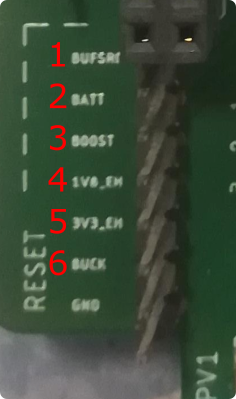
\includegraphics[width=0.15\textwidth]{figs/reset-procedure.png}
    \caption{RESET pin headers.}
    \label{fig:reset-procedure}
\end{figure}

\begin{figure}[h!]
    \centering
    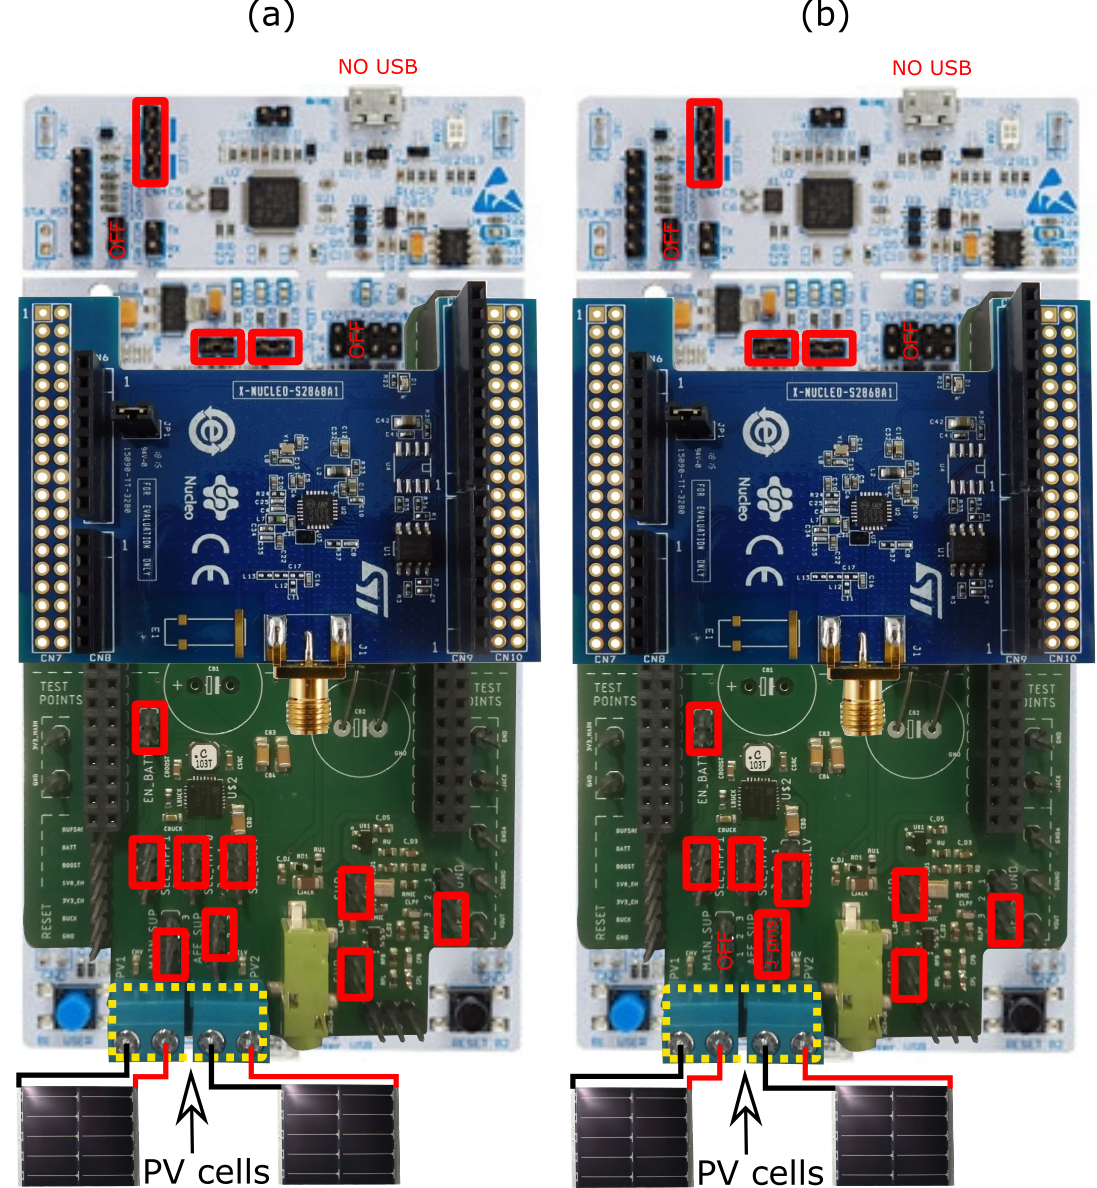
\includegraphics[width=0.7\textwidth]{figs/settings-mode-eh.png}
    \caption{Settings for the boards, EH mode. It is possible to supply all boards at once with (a) 3V3\_EH and (b) 1V8\_EH. Be careful to set properly all jumpers.}
    \label{fig:settings-mode-eh}
\end{figure}

\begin{bclogo}[couleur = gray!20, arrondi = 0.2, logo=\bcinfo]{Supplying the system at 1V8 with EH}
You can enable the 1V8 LDO output from the energy harvesting chip by changing the jumper SEL\_ENLV as presented in Table \ref{tab:EH-headers}. You can then chose to supply the whole system with that 1V8 source. To do this, make sure the MAIN\_SUP jumper is OFF and then, use a 3-pins jumper that we can provide you (on demand!) to connect the 3 pins of the AFE\_SUP together, as shown in Fig. \ref{fig:settings-mode-eh}b. \textbf{Important}: do not put anything else than the PV cells in the blue connectors !
\end{bclogo}
